\documentclass[tikz, convert = false]{standalone}%

\usepackage[utf8]{inputenx}%  http://ctan.org/pkg/inputenx
% Euler for math | Palatino for rm | Helvetica for ss | Courier for tt
\renewcommand{\rmdefault}{ppl}% rm
\linespread{1.05}% Palatino needs more leading
\usepackage[scaled]{helvet}% ss //  http://ctan.org/pkg/helvet
\usepackage{courier}% tt // http://ctan.org/pkg/courier
\usepackage{eulervm}  %  http://ctan.org/pkg/eulervm
% a better implementation of the euler package (not in gwTeX)
\normalfont%
\usepackage[T1]{fontenc}%  http://ctan.org/pkg/fontenc
\usepackage{textcomp}%  http://ctan.org/pkg/textcomp

\begin{document}
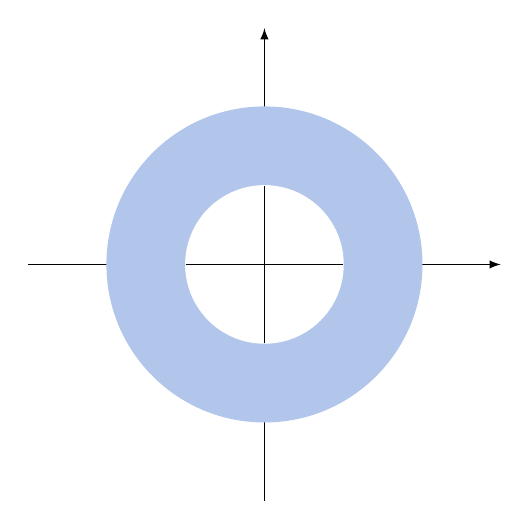
\begin{tikzpicture}
  \draw[-latex] (-3, 0) -- (3, 0);
  \draw[-latex] (0, -3) -- (0, 3);

  \filldraw[blue!75!green!30] (0, 0) circle[radius = 2];
  \filldraw[white] (0, 0) circle[radius = 1];

  \draw (-1, 0) -- (1, 0);
  \draw (0, -1) -- (0, 1);
\end{tikzpicture}
\end{document}
%%% Local Variables:
%%% mode: latex
%%% TeX-master: t
%%% End:
